% latex table generated in R 3.6.3 by xtable 1.8-4 package
% Thu Jan 18 11:46:57 2024
\begin{table}[ht]
\centering
\begin{tabular}{rlrrr}
  \hline
 & OTU & MeanRA & MedianRA & SE \\ 
  \hline
2493093 & Bradyrhizobium sp. LCT & 0.00006056 & 0.00005830 & 0.00000524 \\ 
  431944 & Magnetospirillum gryphiswaldense & 0.00007752 & 0.00007728 & 0.00000415 \\ 
  634177 & Komagataeibacter medellinensis & 0.00004838 & 0.00004750 & 0.00000199 \\ 
  33995 & Komagataeibacter europaeu & 0.00004065 & 0.00004060 & 0.00000282 \\ 
  2558360 & Oecophyllibacter saccharovoran & 0.00005341 & 0.00005566 & 0.00000247 \\ 
  2587846 & Roseovarius sp. THAF & 0.00005176 & 0.00005216 & 0.00000235 \\ 
  92947 & Ketogulonicigenium robustu & 0.00008052 & 0.00008249 & 0.00000298 \\ 
  314260 & Parvularcula bermudensis & 0.00007436 & 0.00007563 & 0.00000399 \\ 
  1207504 & Burkholderia pseudomultivoran & 0.00005497 & 0.00005810 & 0.00000372 \\ 
  1637853 & Burkholderia sp. NRF60-BP & 0.00007118 & 0.00007057 & 0.00000385 \\ 
  521 & Bordetella aviu & 0.00006417 & 0.00007302 & 0.00000989 \\ 
  1235827 & Herbaspirillum rubrisubalbicans & 0.00006018 & 0.00005809 & 0.00000303 \\ 
  1881017 & Pseudomonas sp. 7SR & 0.00008136 & 0.00006981 & 0.00001003 \\ 
  2726956 & Pseudomonas sp. MSPm & 0.00008273 & 0.00006017 & 0.00001774 \\ 
  2730847 & Pseudomonas sp. ADAK1 & 0.00004755 & 0.00004589 & 0.00000504 \\ 
  1898684 & Pseudomonas sp. LPH & 0.00004990 & 0.00002507 & 0.00001502 \\ 
  86185 & Pseudomonas lundensi & 0.00005400 & 0.00004848 & 0.00000507 \\ 
  50340 & Pseudomonas fuscovagina & 0.00002563 & 0.00002252 & 0.00000237 \\ 
  1301098 & Pseudomonas knackmussii & 0.00005705 & 0.00005269 & 0.00000606 \\ 
  46677 & Pseudomonas agaric & 0.00005431 & 0.00004376 & 0.00000674 \\ 
  1274359 & Pseudomonas sihuiensi & 0.00004519 & 0.00003314 & 0.00000810 \\ 
  1421430 & Pseudomonas granadensi & 0.00004859 & 0.00004234 & 0.00000648 \\ 
  122355 & Pseudomonas psychrophil & 0.00003259 & 0.00002956 & 0.00000405 \\ 
  64187 & Xanthomonas oryzae & 0.00004085 & 0.00004053 & 0.00000176 \\ 
  1619313 & Duffyella gerundensi & 0.00003629 & 0.00003467 & 0.00000222 \\ 
  180957 & Pectobacterium brasiliens & 0.00002350 & 0.00002387 & 0.00000169 \\ 
  158850 & Providencia rustigiani & 0.00000538 & 0.00000518 & 0.00000090 \\ 
  38313 & Shewanella alga & 0.00002941 & 0.00003023 & 0.00000170 \\ 
  1630135 & Dermabacter vaginali & 0.00007076 & 0.00006984 & 0.00000509 \\ 
  401472 & Corynebacterium ureicelerivoran & 0.00006434 & 0.00006708 & 0.00000361 \\ 
  79604 & Denitrobacterium detoxifican & 0.00004760 & 0.00005318 & 0.00000407 \\ 
  37482 & Laceyella sacchar & 0.00004591 & 0.00003736 & 0.00000930 \\ 
  1363 & Lactococcus garviea & 0.00000714 & 0.00000582 & 0.00000144 \\ 
  1932004 & Haloarcula taiwanensi & 0.00003757 & 0.00003976 & 0.00000326 \\ 
  570267 & Methanocella paludicol & 0.00004136 & 0.00004163 & 0.00000310 \\ 
   \hline
\end{tabular}
\caption{Keystone OTUs of } 
\end{table}
\begin{figure}
\centering
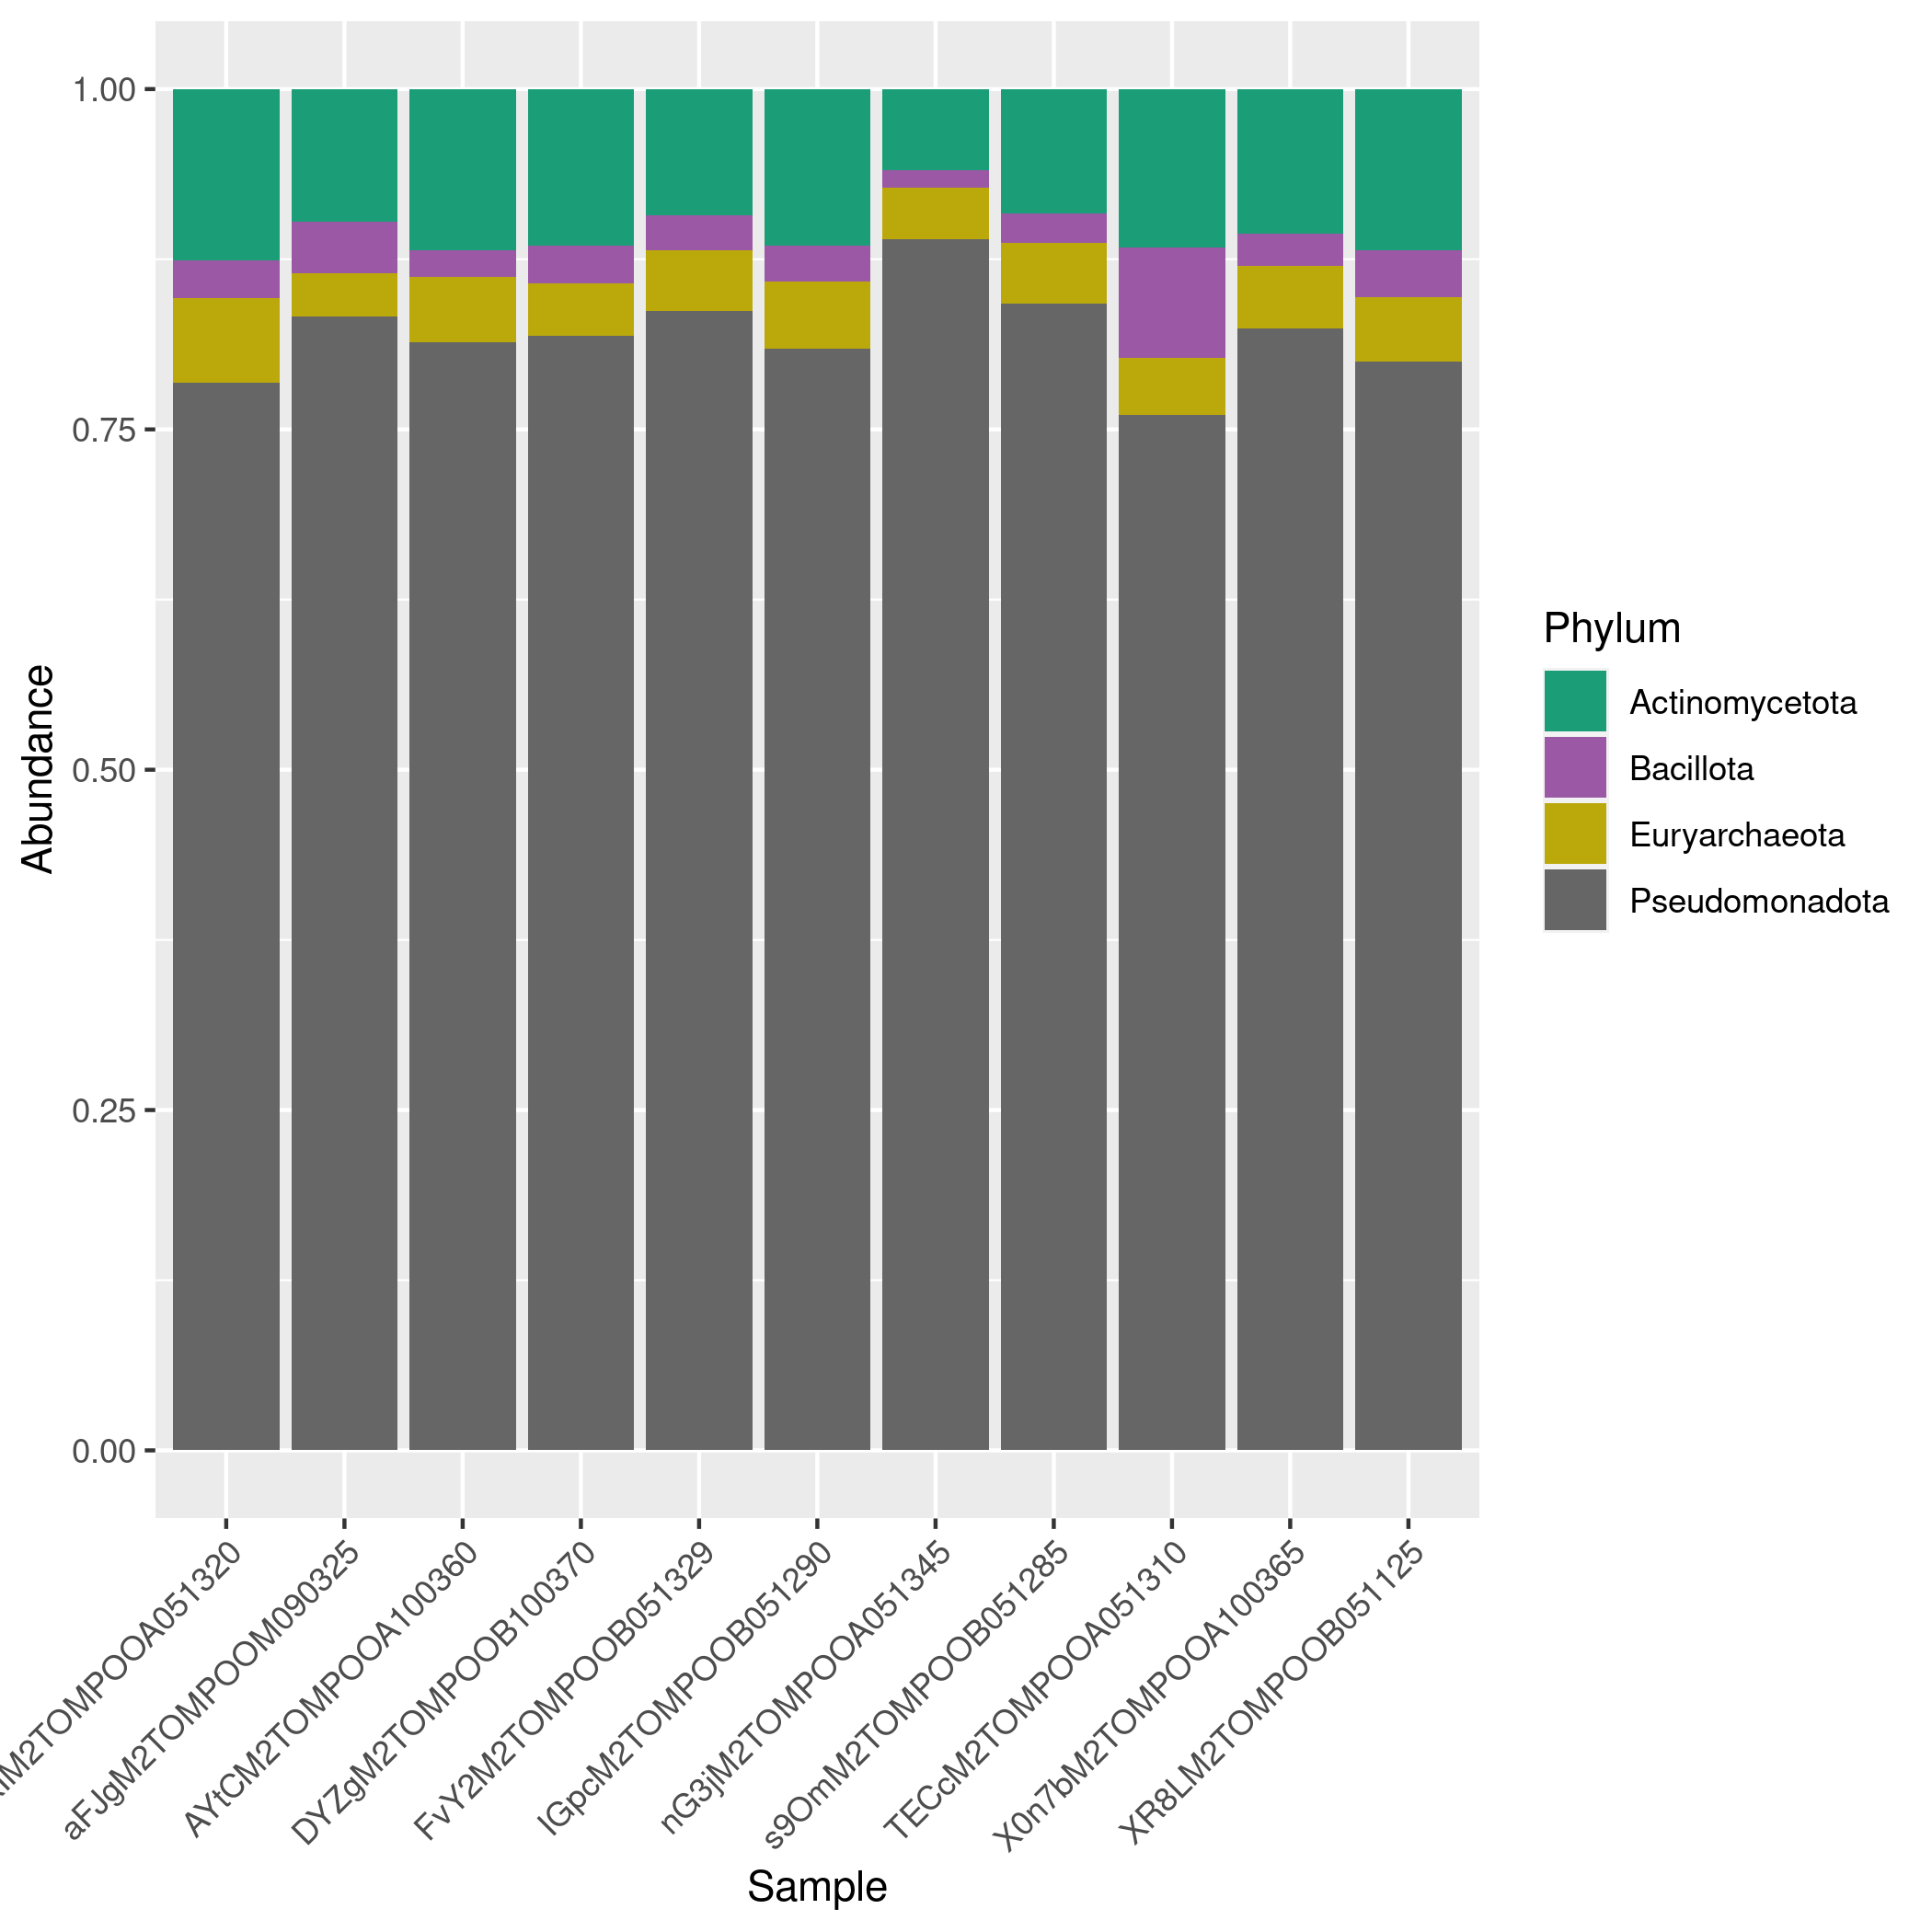
\includegraphics[scale = 0.8]{tomate_aleatorio1_3.csv_relative_abundance_Phylum.png}
\caption{Relative abundance by phyla of keystone OTUs }
\label{fig:tomate_aleatorio1_3.csv_phyla}
\end{figure}
\begin{figure}
\centering
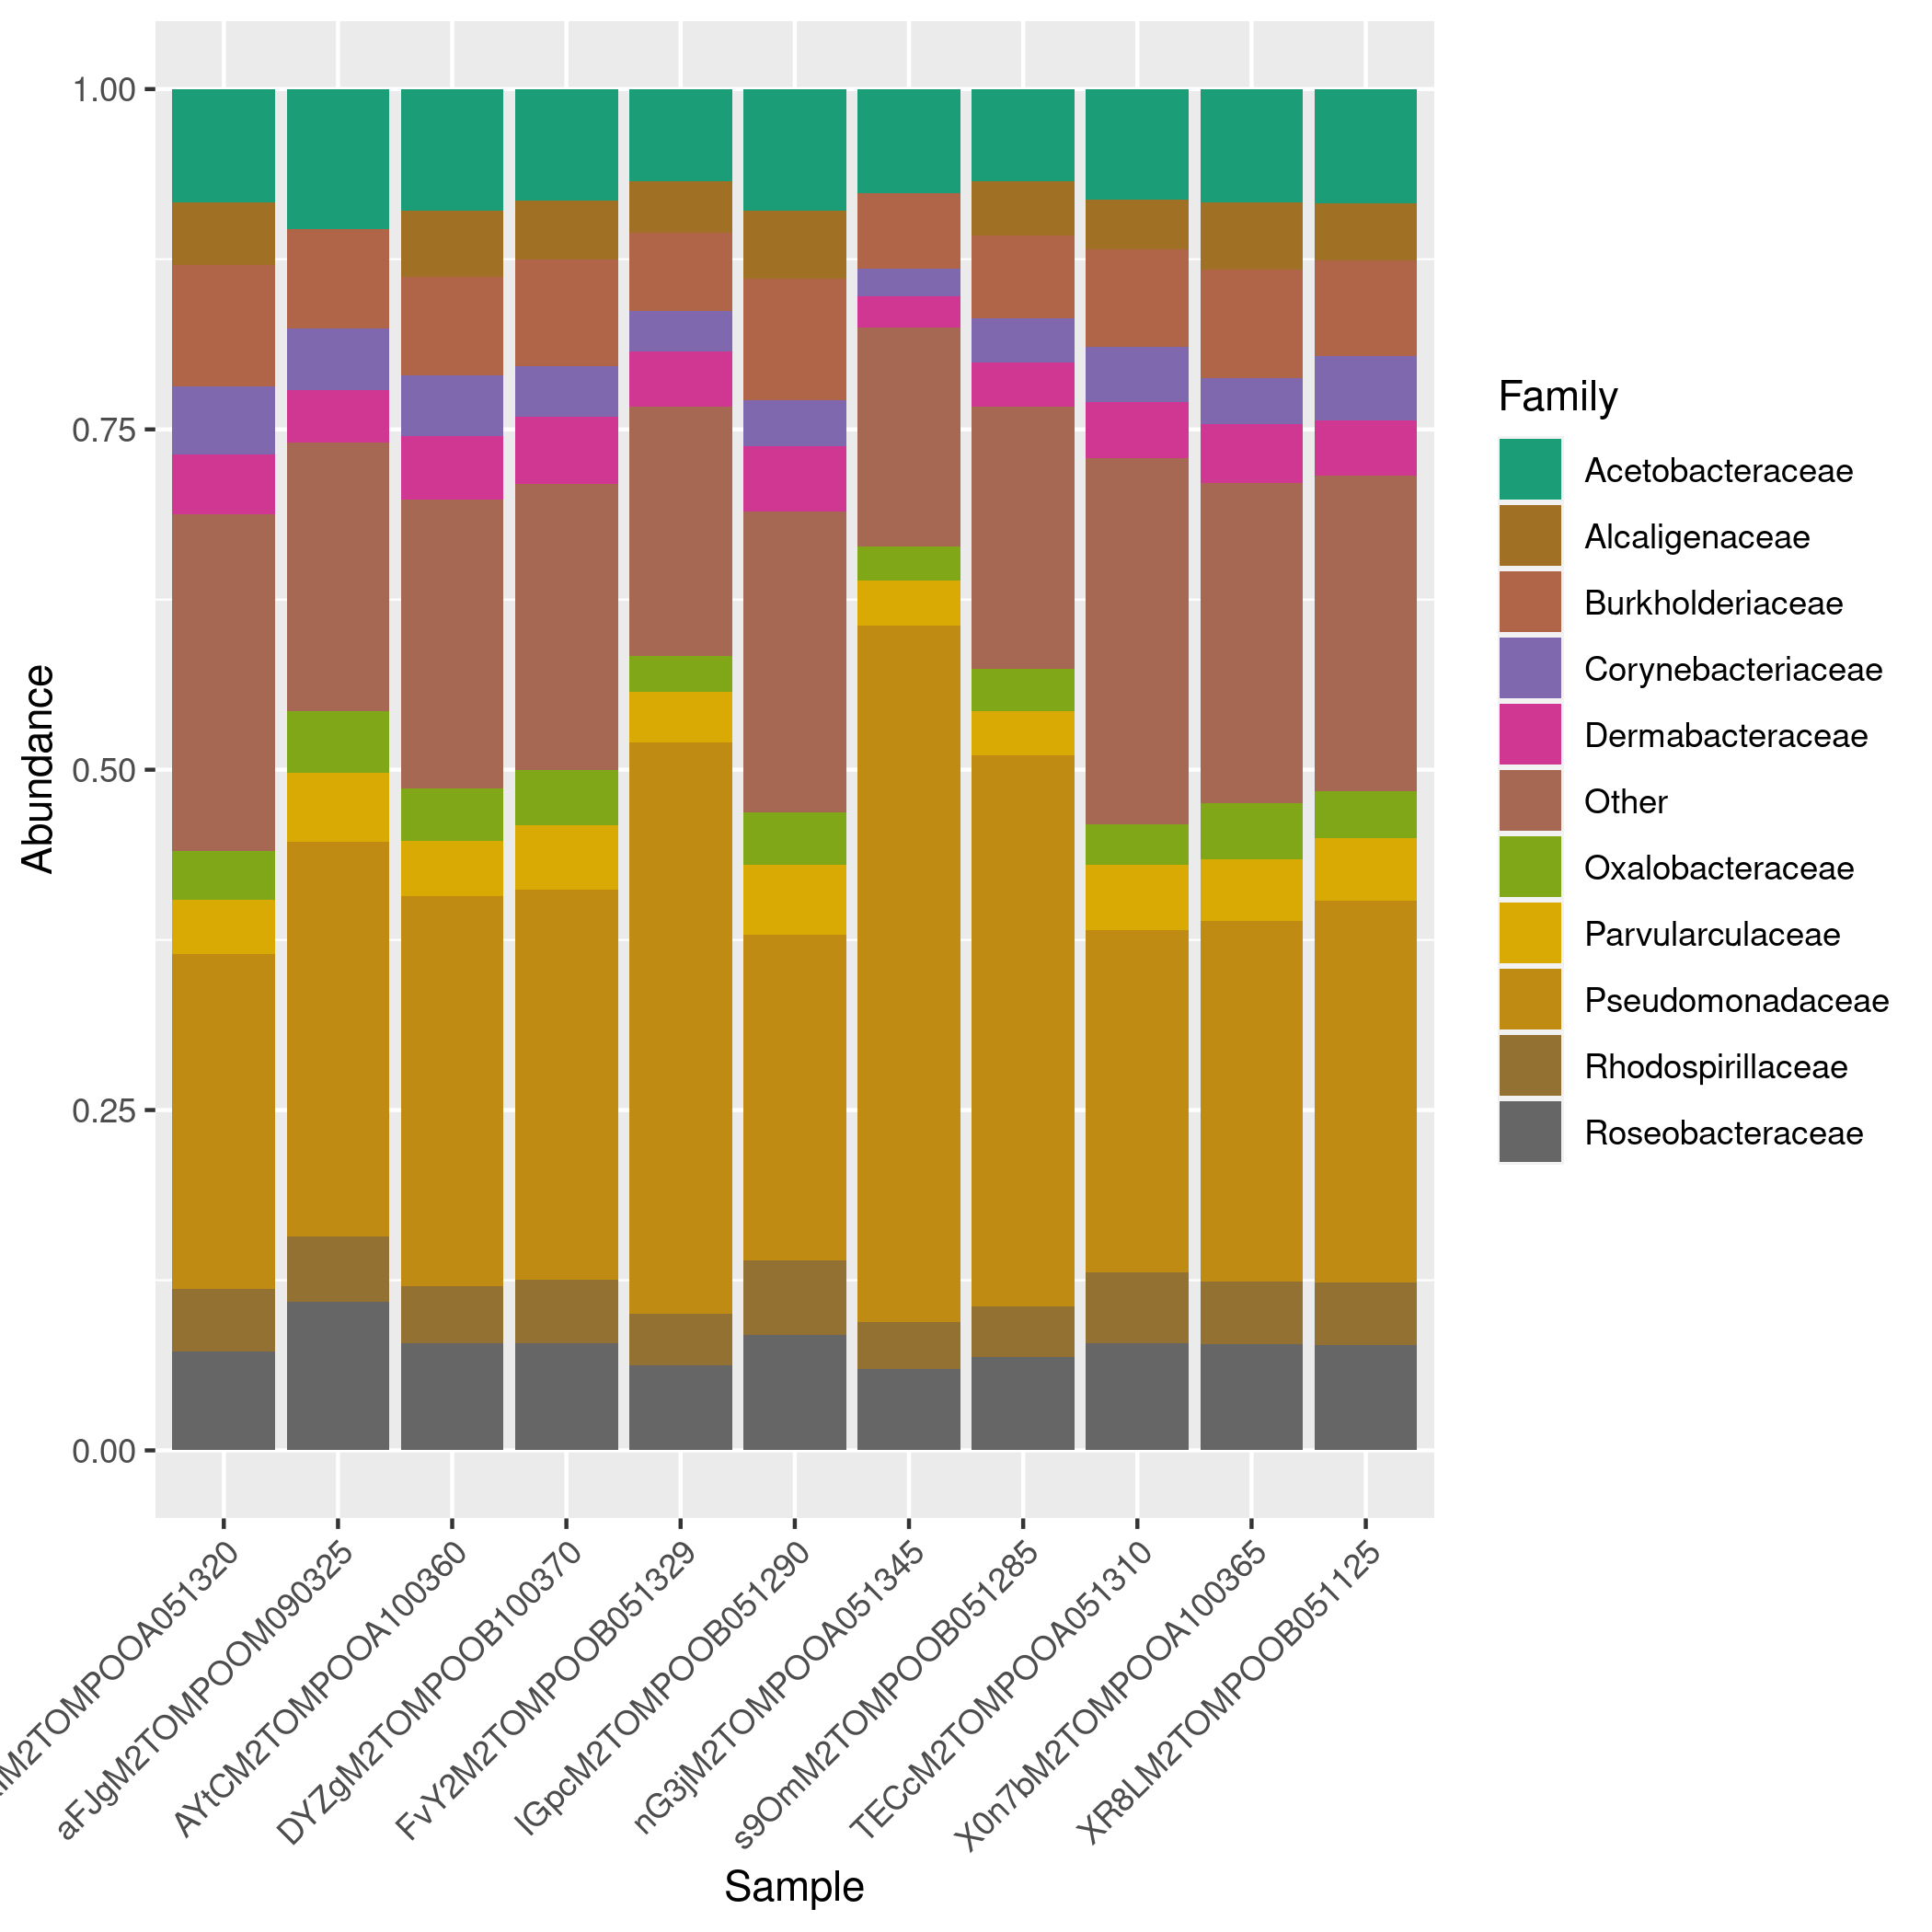
\includegraphics[scale = 0.8]{tomate_aleatorio1_3.csv_relative_abundance_Family.png}
\caption{Relative abundance by families of keystone OTUs }
\label{fig:tomate_aleatorio1_3.csv_family}
\end{figure}
\begin{figure}
\centering
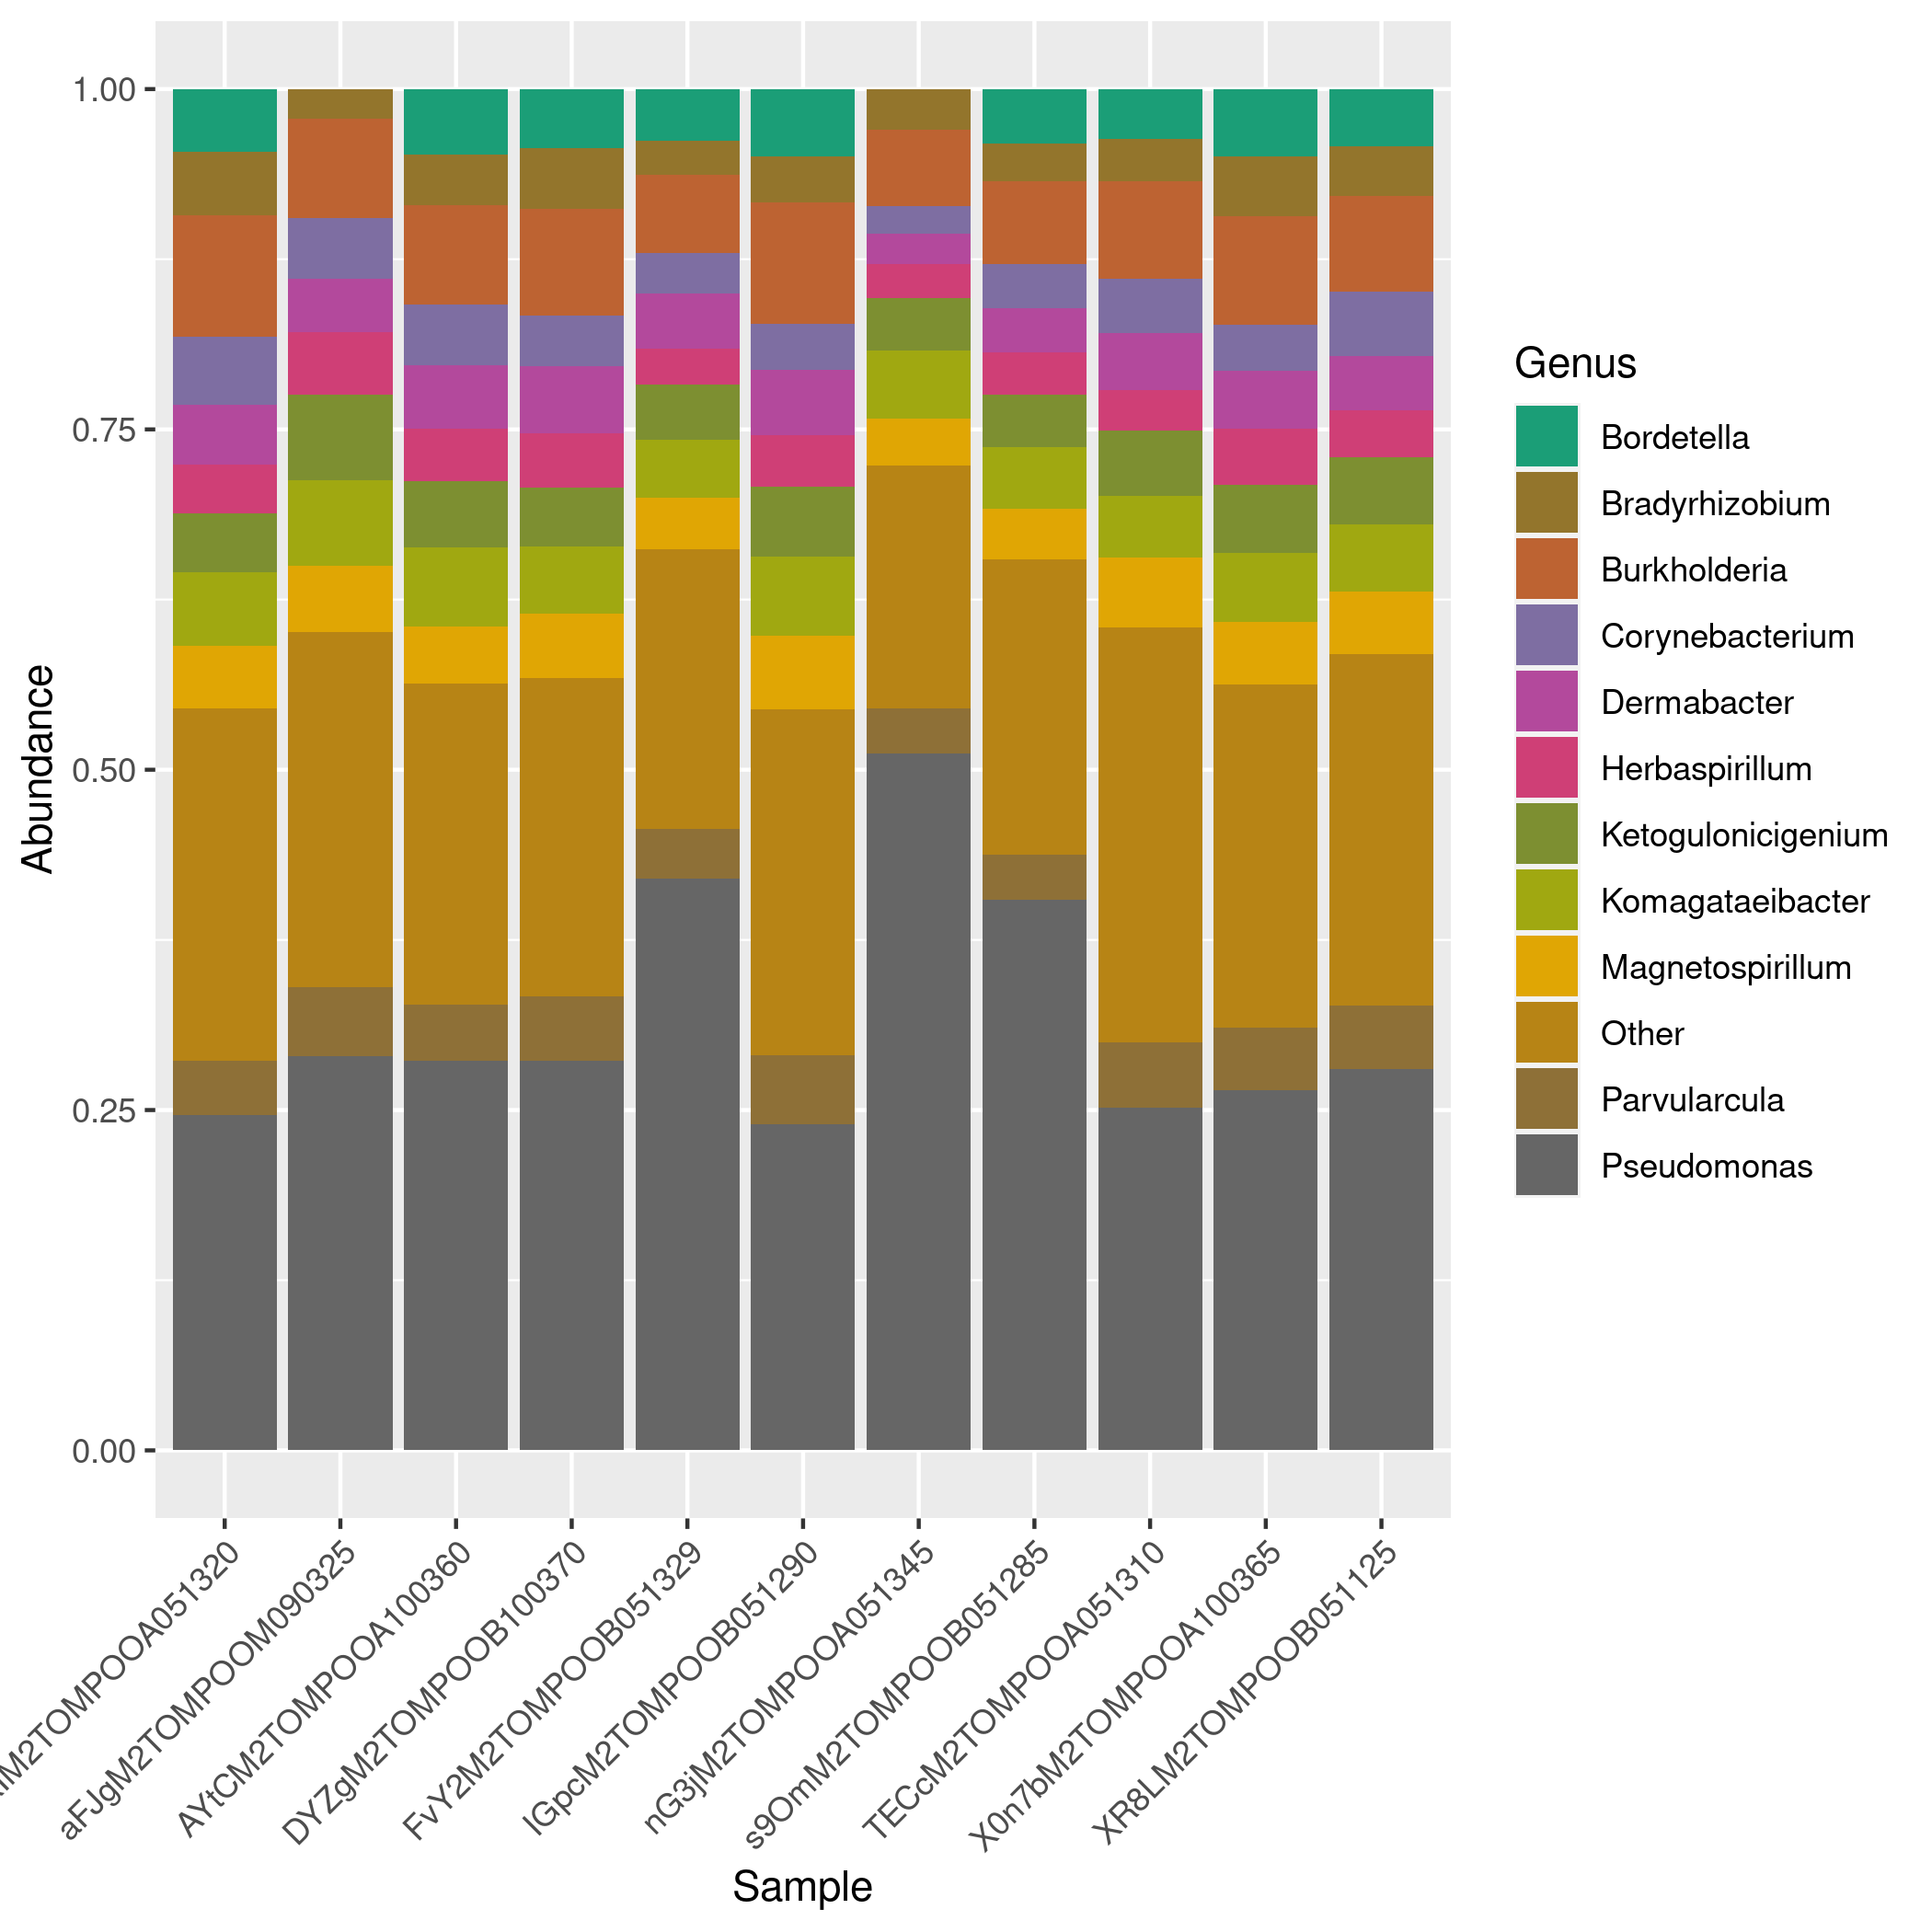
\includegraphics[scale = 0.8]{tomate_aleatorio1_3.csv_relative_abundance_Genus.png}
\caption{Relative abundance by genera of keystone OTUs }
\label{fig:tomate_aleatorio1_3.csv_genus}
\end{figure}
\begin{figure}
   \centering
   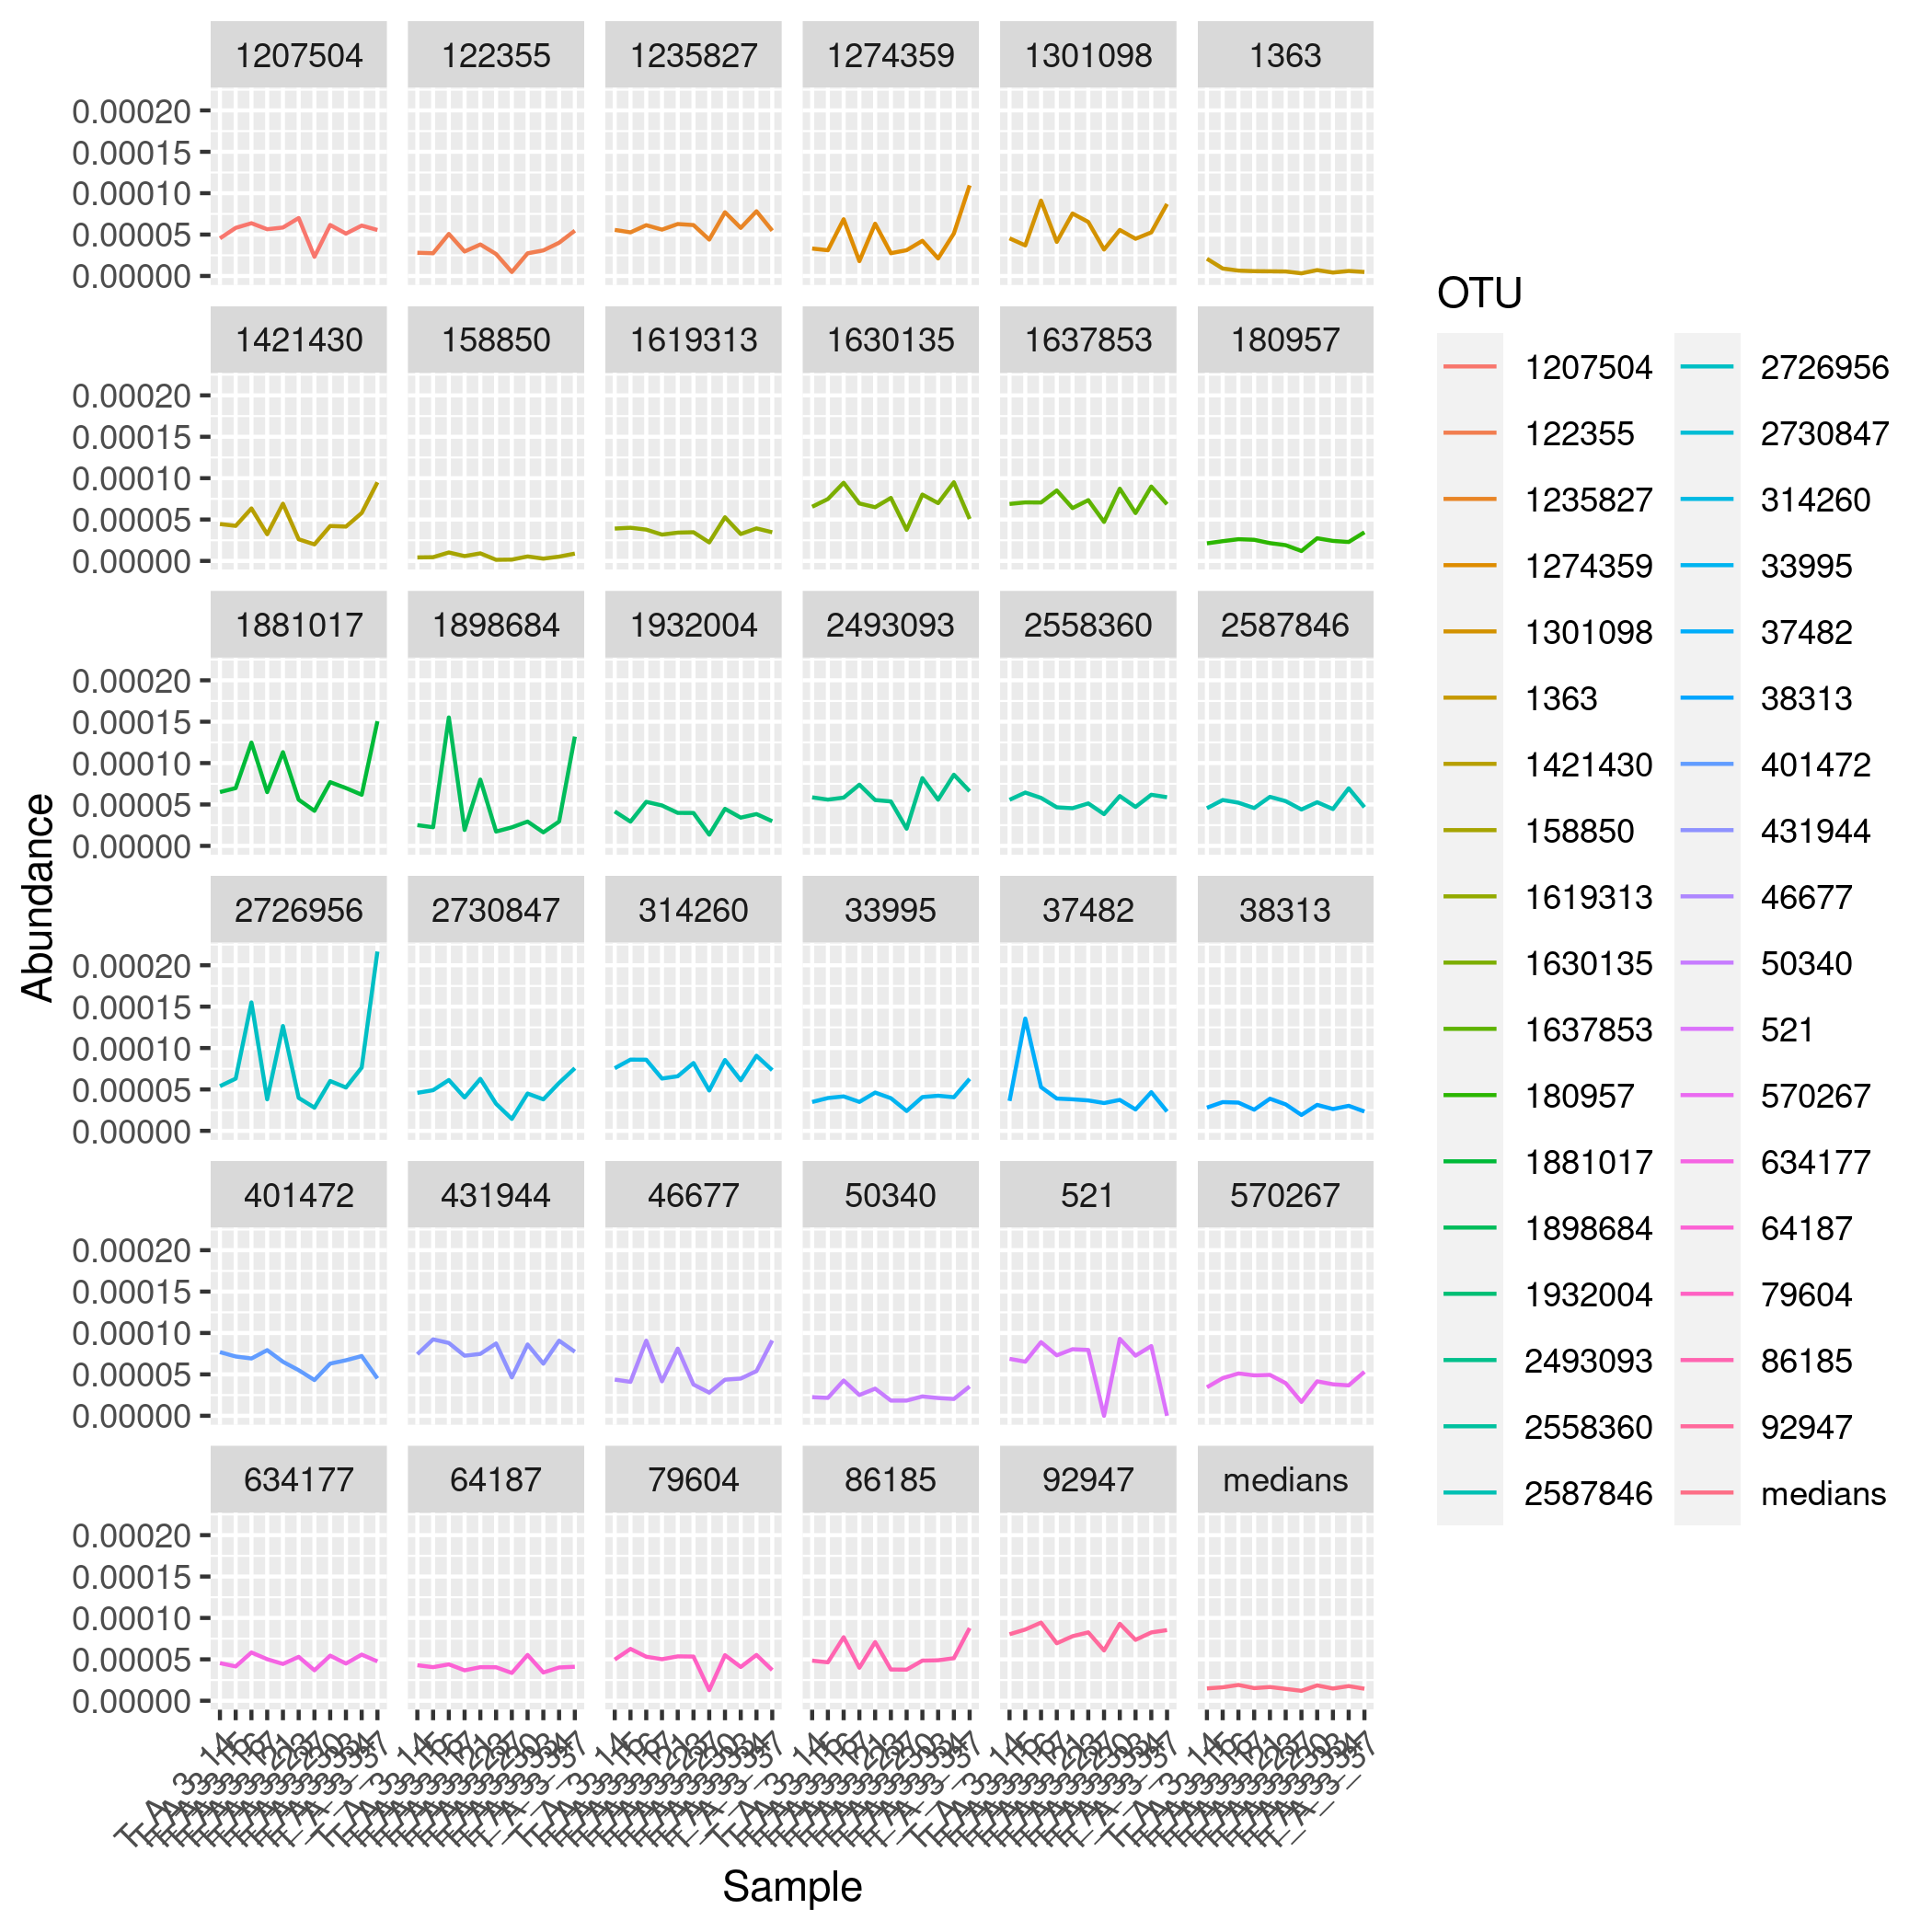
\includegraphics[scale = 0.8]{abundance_tomate_aleatorio1_3.csv_key_otus_medians.png}
   \caption{Plots representing relative abundance of each keystone OTU and one representing the median relative abundance  across samples of rhizosphere of tomate_aleatorio1_3.csv. Most keystone OTUs have relative abundance bigger than the median across all samples.  }
   \label{key_otus_vs_medians_tomate_aleatorio1_3.csv}
\end{figure}
\begin{figure}
 \centering
 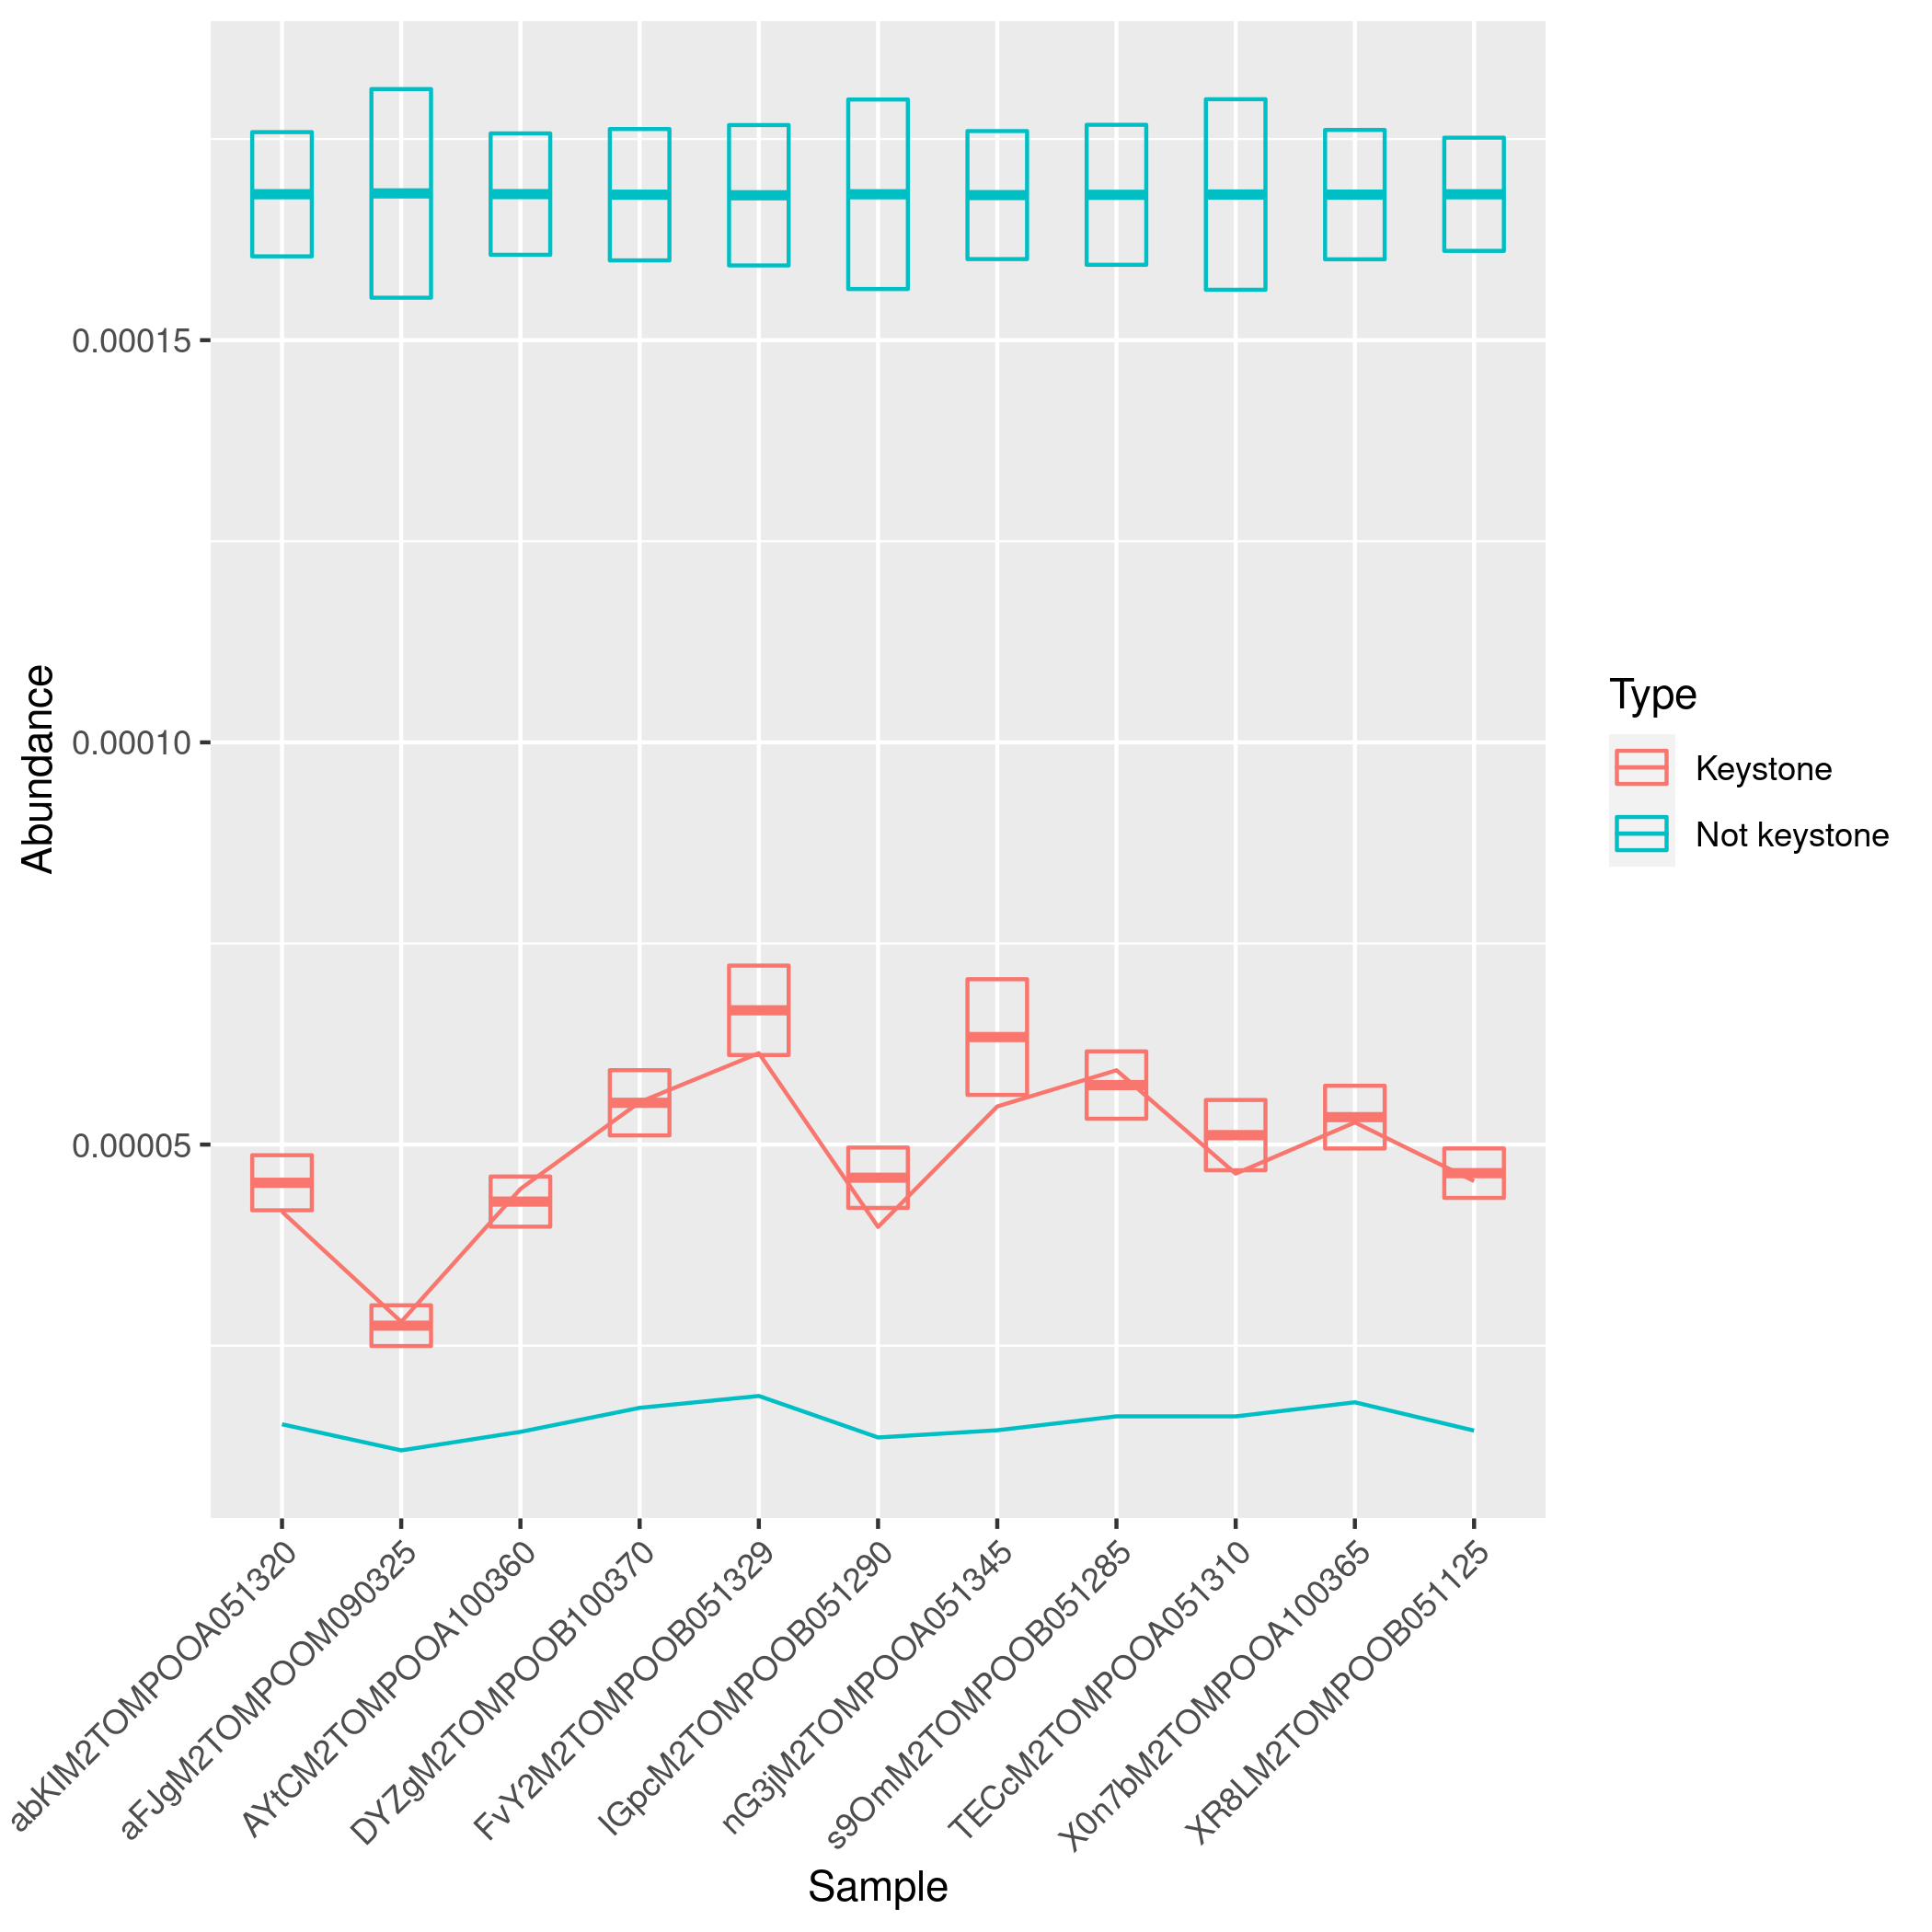
\includegraphics[scale = 0.75]{mean_median_key_vs_not_key_tomate_aleatorio1_3.csv.png}
\caption{Boxes represent mean and standard error in the distribution of corresponding samples. Lines represent the corresponding medians. In these samples of rhizosphere oftomate_aleatorio1_3.csv}
\label{mean_median_tomate_aleatorio1_3.csv}
\end{figure}
\begin{figure}
   \centering
   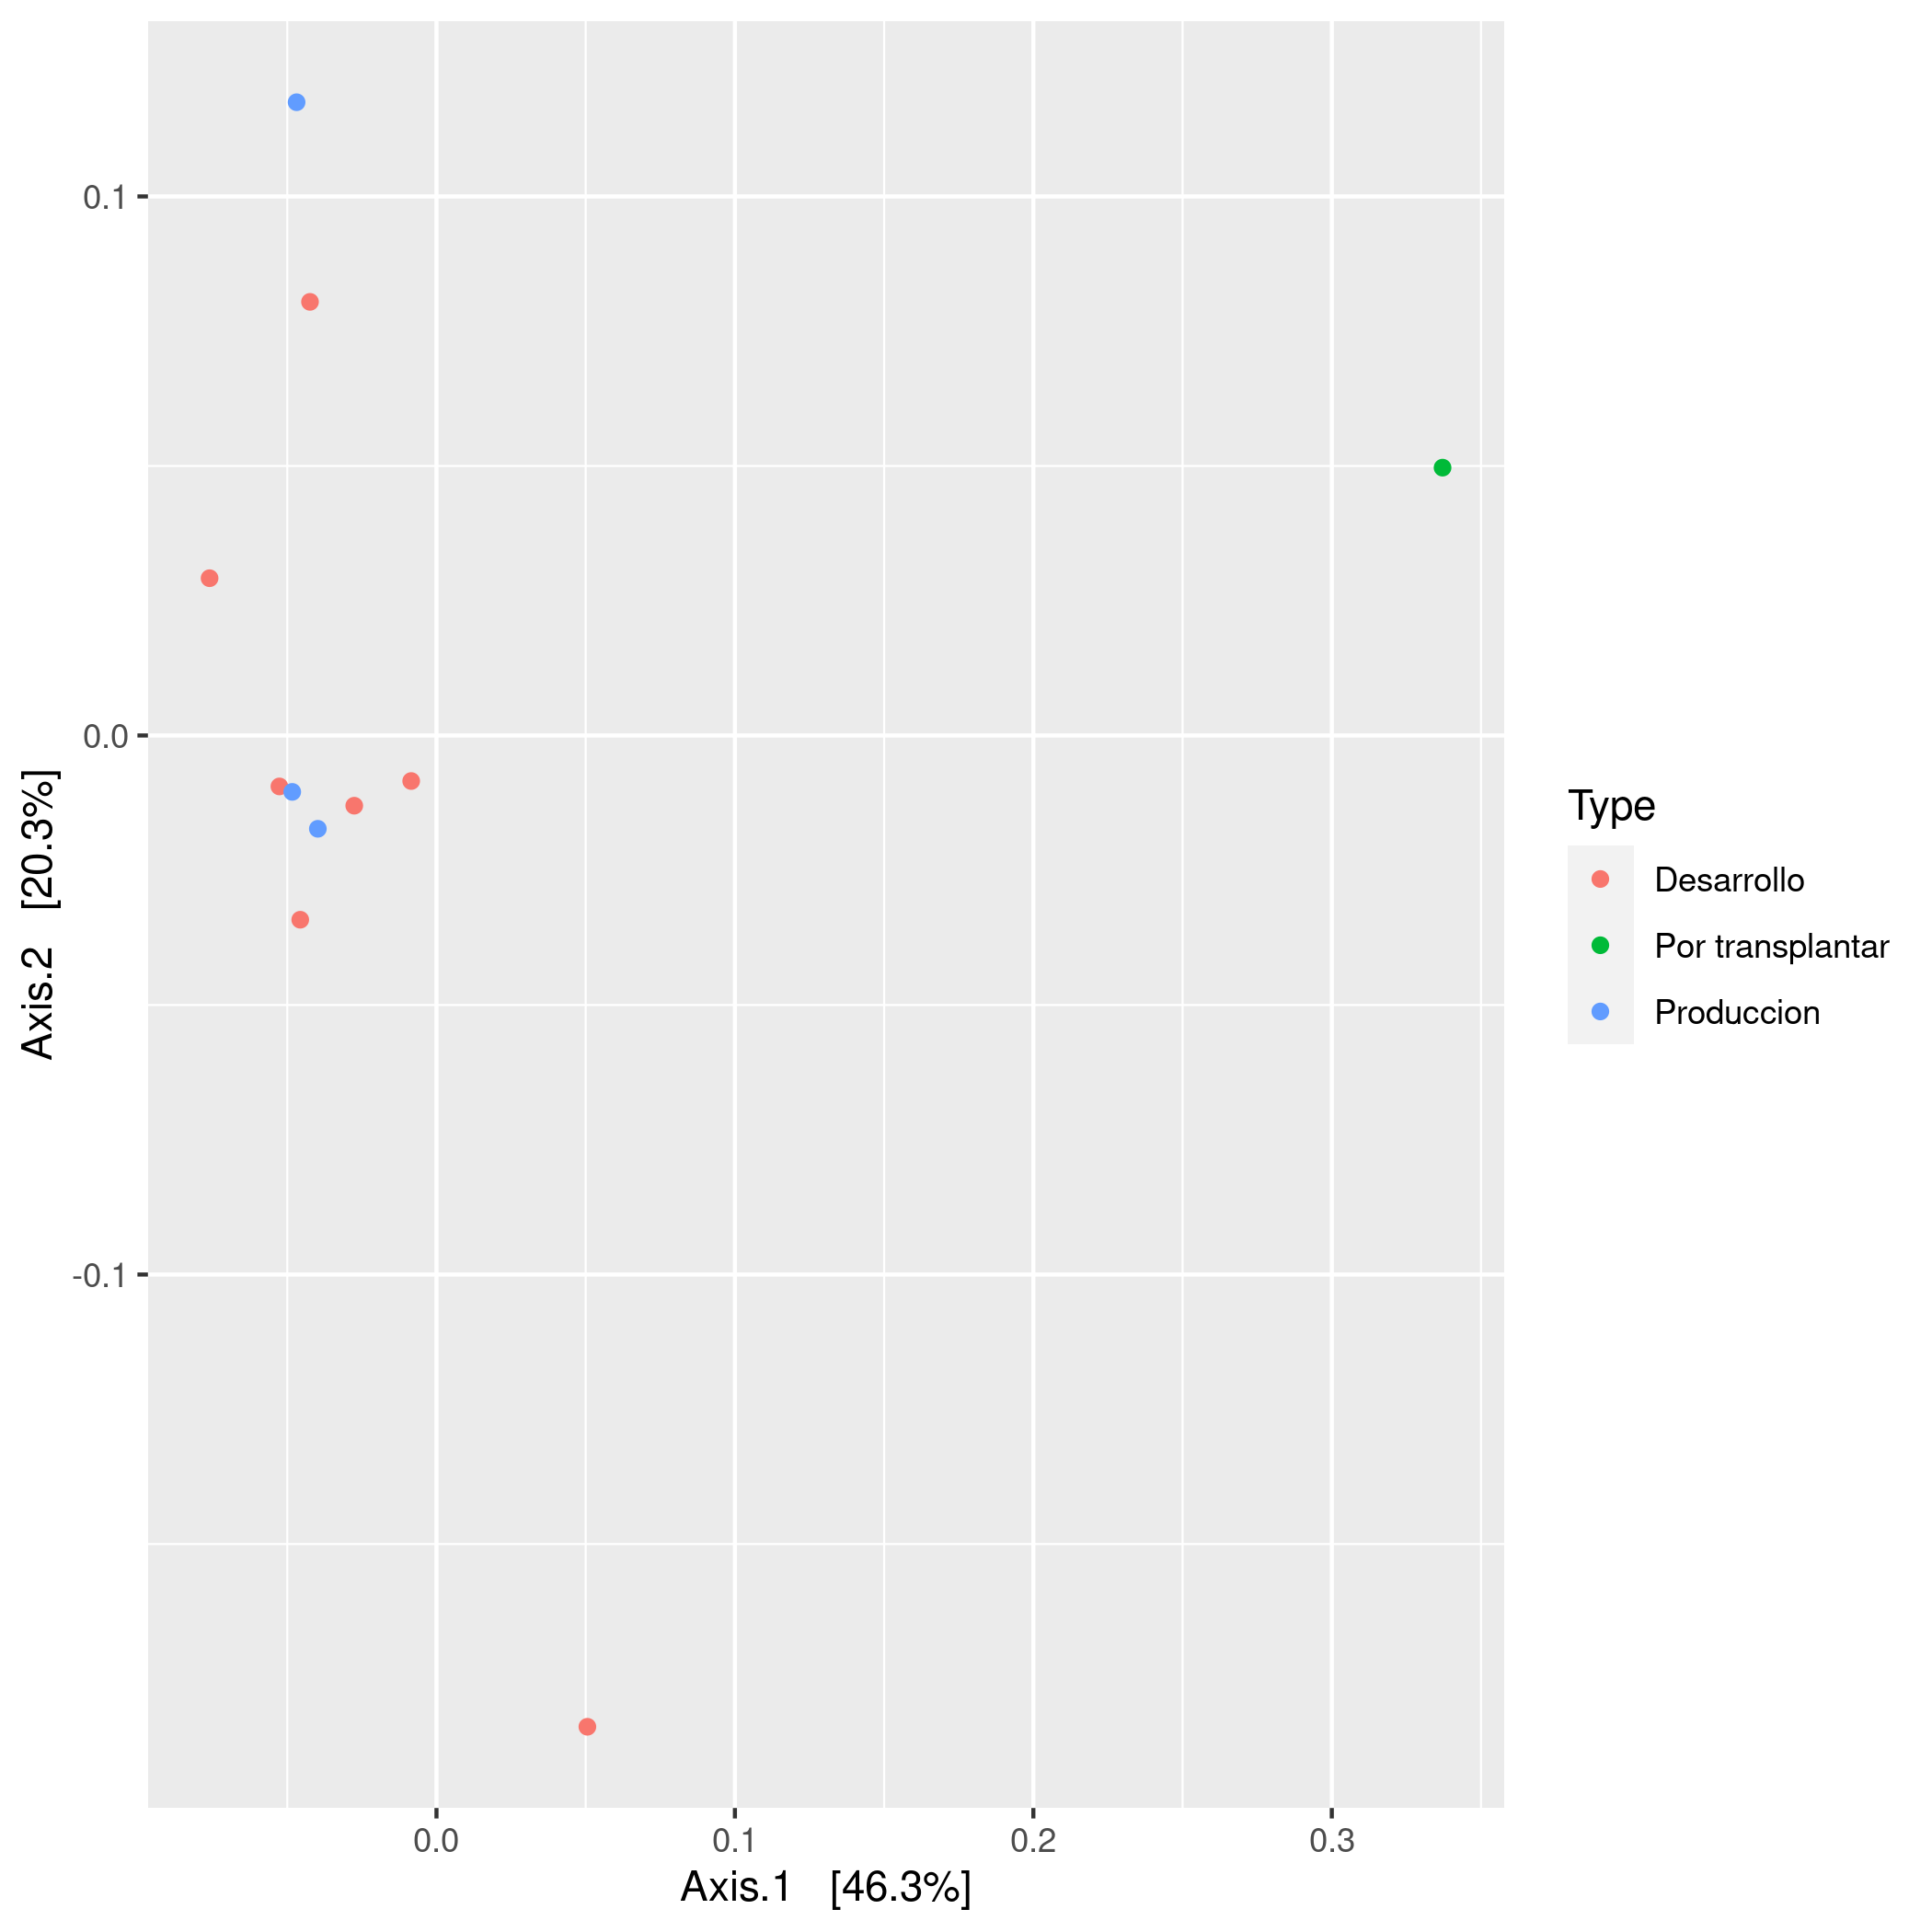
\includegraphics[scale = 0.7]{pcoa_muestras_tomate_aleatorio1_3.csv.png}
 \caption{PCoA analysis with Bray-Curtis distance of rhizosphere samples of tomate_aleatorio1_3.csv.}
 \label{fig:tomate_aleatorio1_3.csv_pcoa}
\end{figure}
\begin{figure}
  \centering
  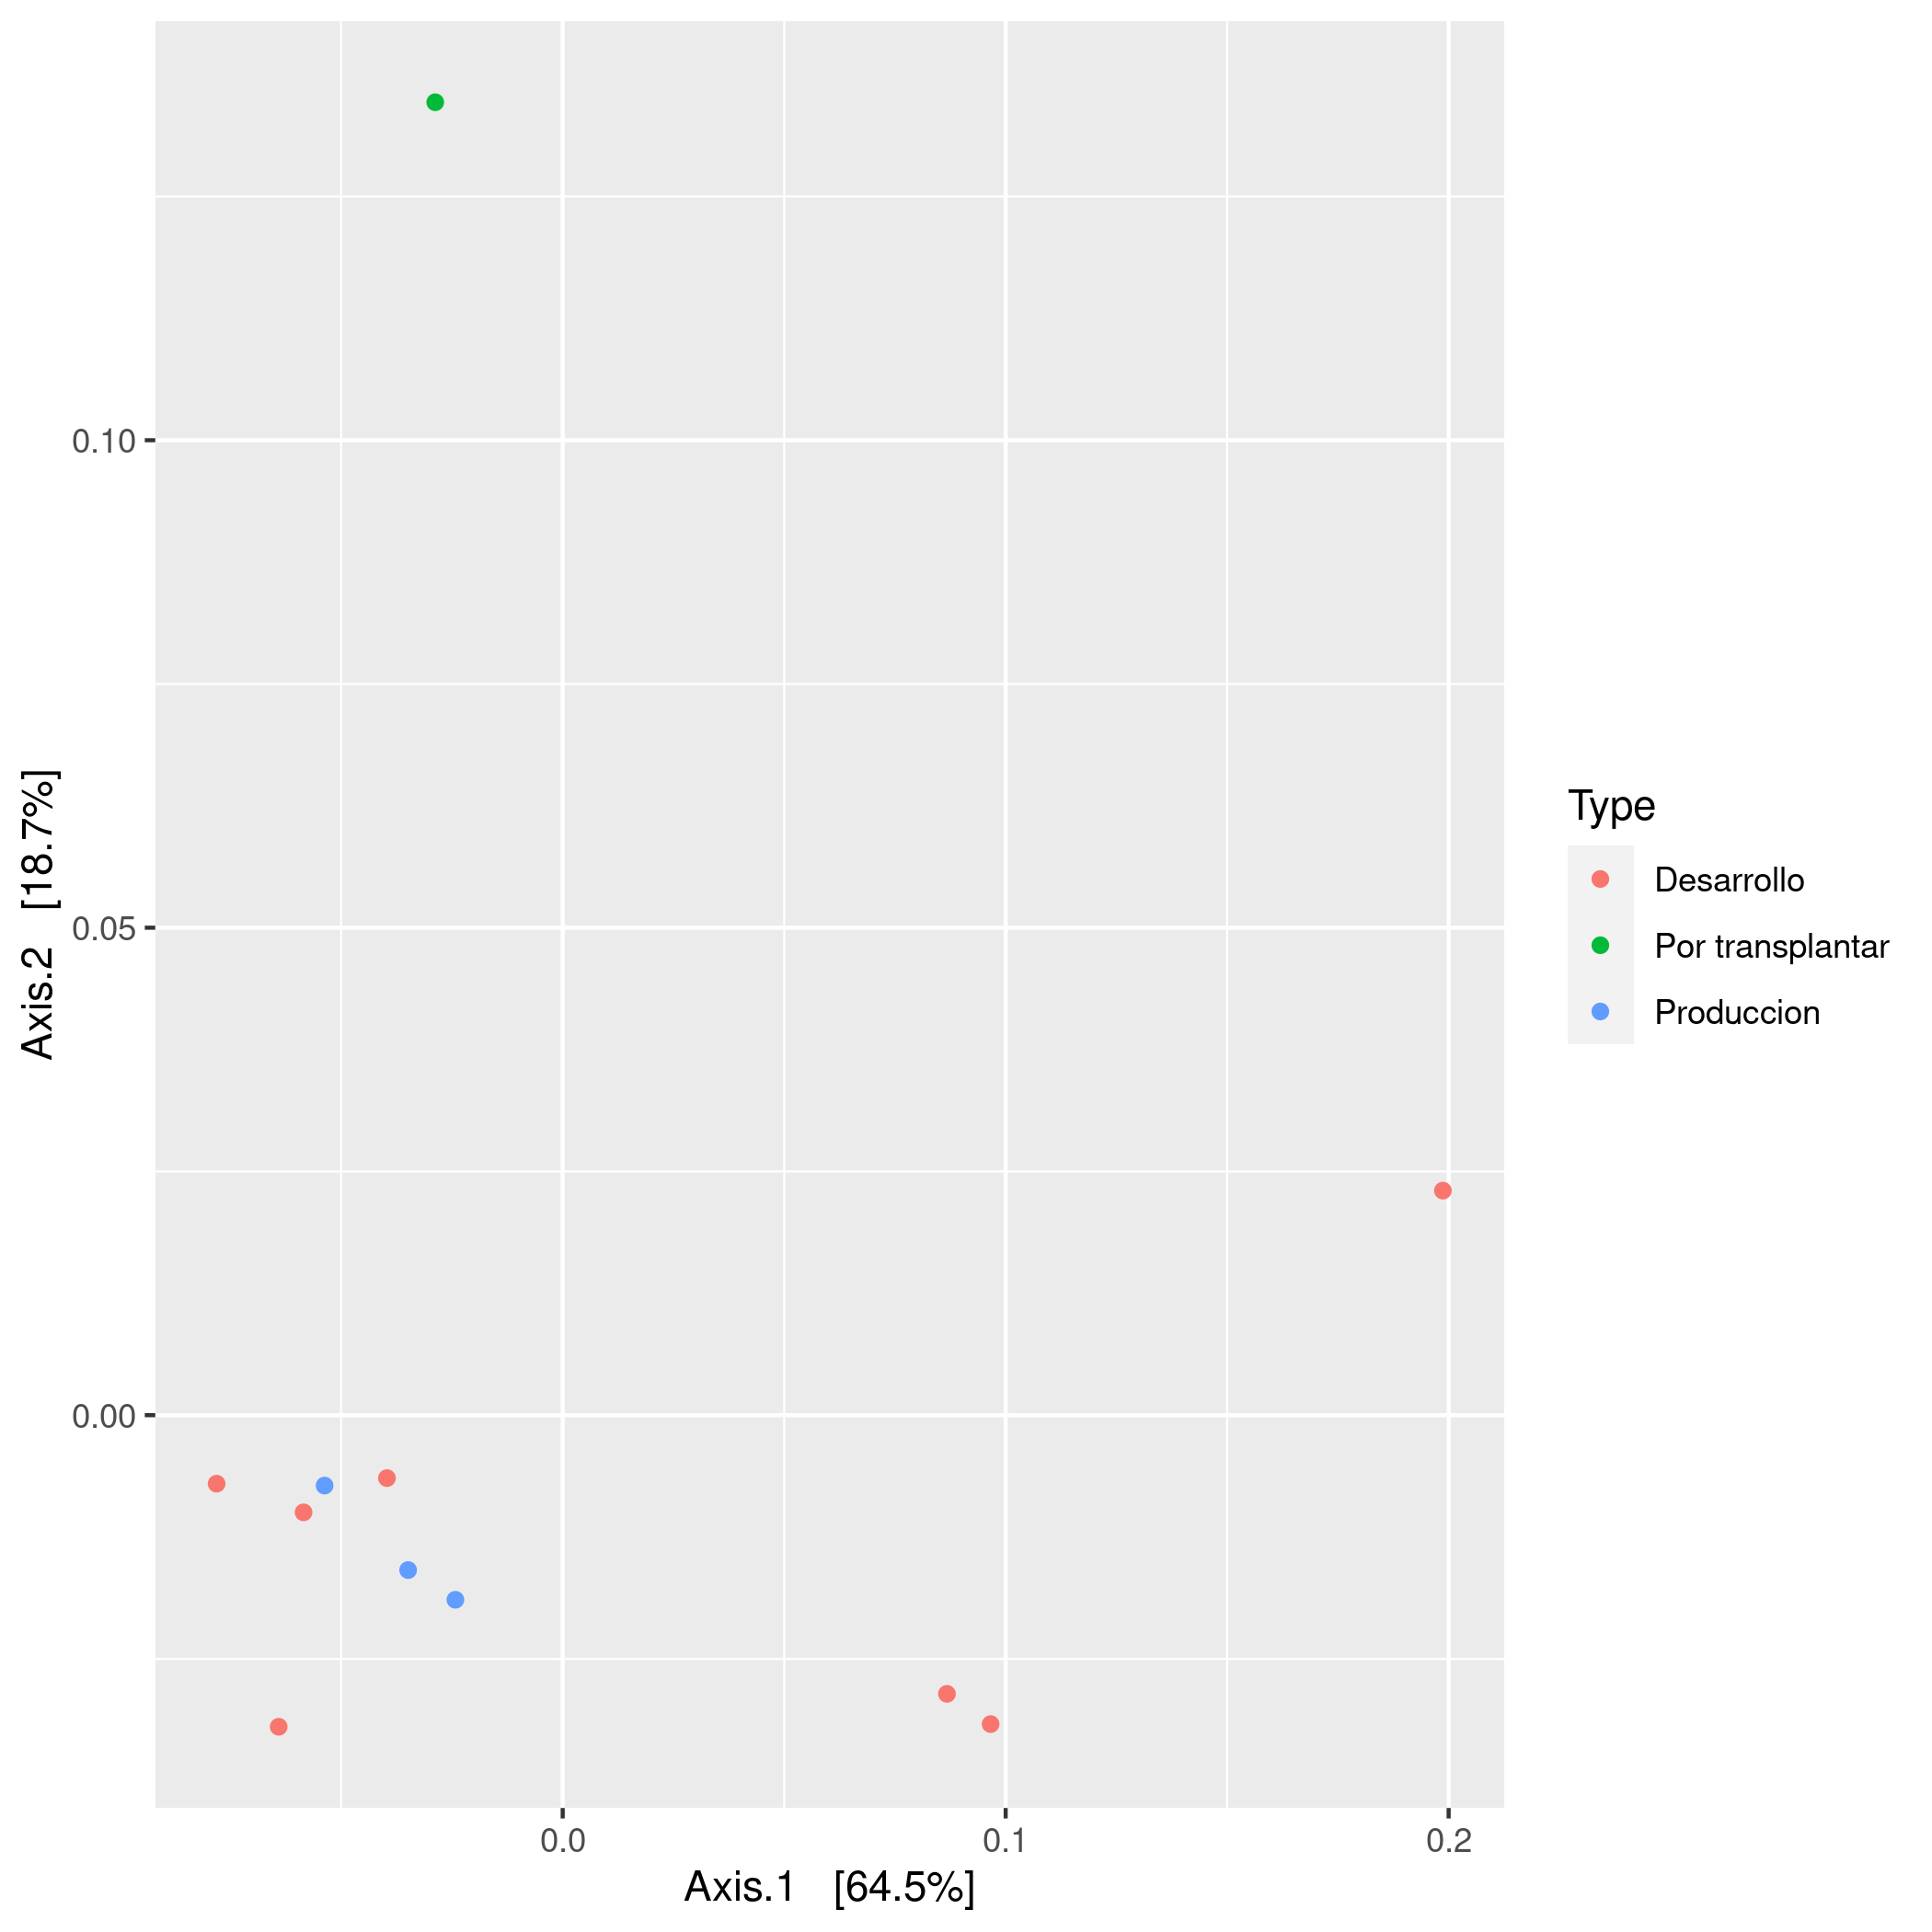
\includegraphics[scale = 0.7]{pcoa_key_otus_tomate_aleatorio1_3.csv.png}
  \caption{PCoA analysis with Bray-Curtis distance of rhizosphere samples of tomate_aleatorio1_3.csv, restricted to keystone OTUs.}
  \label{fig:tomate_aleatorio1_3.csv_pcoa_key_otus}
\end{figure}
